% Raster images, TikZ drawings with text labels, pgfplots.
\documentclass{beamer}
\usepackage{tikz}
\usepackage{pgfplots}
\pgfplotsset{compat=1.18}
\title{Figures}
\author{Tester}
\date{}

\begin{document}

\begin{frame}{Raster image with caption}
  \centering
  \includegraphics[width=0.6\textwidth]{example-image-a}

  An image caption below the picture.
\end{frame}

\begin{frame}{TikZ diagram with labels}
  \centering
  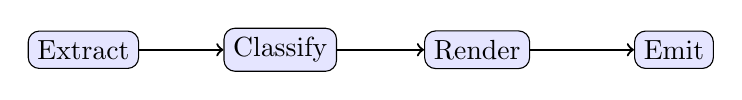
\begin{tikzpicture}[node distance=2.5cm, every node/.style={draw, rounded corners, fill=blue!10}]
    \node (a) {Extract};
    \node[right of=a] (b) {Classify};
    \node[right of=b] (c) {Render};
    \node[right of=c] (d) {Emit};
    \draw[->, thick] (a) -- (b);
    \draw[->, thick] (b) -- (c);
    \draw[->, thick] (c) -- (d);
  \end{tikzpicture}

  \vspace{1em}
  Text below the diagram should become a text box, but the node labels should not.
\end{frame}

\begin{frame}{Plot next to bullets}
  \begin{columns}
    \column{0.5\textwidth}
    \begin{itemize}
      \item The plot on the right
      \item has axis tick labels
      \item that are PDF text
    \end{itemize}
    \column{0.5\textwidth}
    \begin{tikzpicture}
      \begin{axis}[width=\linewidth, xlabel=$x$, ylabel=$y$]
        \addplot[blue, domain=0:4] {x^2};
      \end{axis}
    \end{tikzpicture}
  \end{columns}
\end{frame}

\begin{frame}{Two images side by side}
  \includegraphics[width=0.45\textwidth]{example-image-b}\hfill
  \includegraphics[width=0.45\textwidth]{example-image-c}
\end{frame}

% A tick row longer than a short label: left as text it made the chart an overlay that emit
% moved and stretched after Slides' words.
\begin{frame}{Long tick labels}
  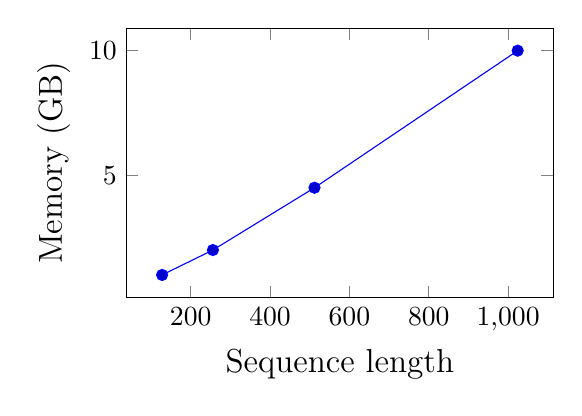
\begin{tikzpicture}
    \begin{axis}[width=7cm, height=5cm, label style={font=\large},
        xlabel={Sequence length}, ylabel={Memory (GB)}]
      \addplot coordinates {(128,1) (256,2) (512,4.5) (1024,10)};
    \end{axis}
  \end{tikzpicture}
\end{frame}

% Titles pushed off their axes are the chart's; the caption under it stays text.
\begin{frame}{Titles pushed away}
  \begin{figure}
    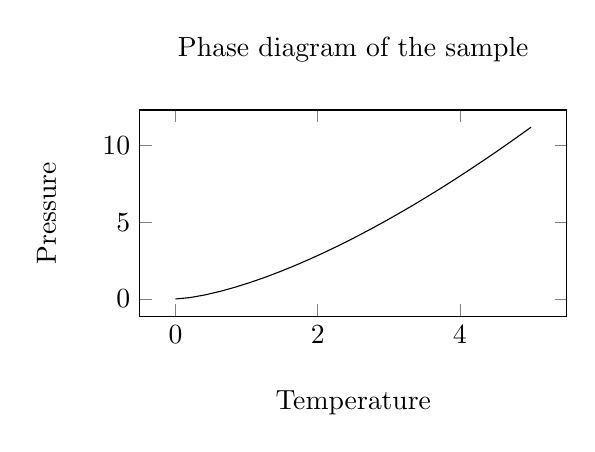
\begin{tikzpicture}
      \begin{axis}[width=7cm, height=4.2cm, xlabel={Temperature}, ylabel={Pressure},
          xlabel style={yshift=-10pt}, ylabel style={yshift=10pt},
          title={Phase diagram of the sample}, title style={yshift=8pt}]
        \addplot[domain=0:5] {x^1.5};
      \end{axis}
    \end{tikzpicture}
    \caption{Measured in the cold room.}
  \end{figure}
\end{frame}

\end{document}
